\documentclass[sigconf]{acmart}

\settopmatter{printacmref=false} % Removes citation information below abstract
%\renewcommand\footnotetextcopyrightpermission[1]{} % removes footnote with conference information in first column
%\pagestyle{plain} % removes running headers

\usepackage{booktabs} % For formal tables
\usepackage{algorithm}
\usepackage[noend]{algpseudocode}

% Copyright
%\setcopyright{none}
%\setcopyright{acmcopyright}
%\setcopyright{acmlicensed}
%\setcopyright{rightsretained}
%\setcopyright{usgov}
%\setcopyright{usgovmixed}
%\setcopyright{cagov}
%\setcopyright{cagovmixed}


% DOI
%\acmDOI{10.475/123_4}

% ISBN
%\acmISBN{123-4567-24-567/08/06}

%Conference
%\acmConference[WOODSTOCK'97]{ACM Woodstock conference}{July 1997}{El
%  Paso, Texas USA} 
%\acmYear{1997}
%\copyrightyear{2016}


%\acmArticle{4}
%\acmPrice{15.00}

% These commands are optional
%\acmBooktitle{Transactions of the ACM Woodstock conference}
%\editor{Jennifer B. Sartor}
%\editor{Theo D'Hondt}
%\editor{Wolfgang De Meuter}

\graphicspath{{./figures/}}

\begin{document}
\title{Breadth First Search on FPGAs: A Pipelined Execution Approach}
%\titlenote{Produces the permission block, and
%  copyright information}
%\subtitle{Extended Abstract}
%\subtitlenote{The full version of the author's guide is available as
%  \texttt{acmart.pdf} document}


\author{     }
%\authornote{Dr.~Trovato insisted his name be first.}
%\orcid{1234-5678-9012}
\affiliation{%
  \institution{   }
%  \streetaddress{P.O. Box 1212}
%  \city{Dublin} 
%  \state{Ohio} 
%  \postcode{43017-6221}
}
\email{       }

%\author{G.K.M. Tobin}
%\authornote{The secretary disavows any knowledge of this author's actions.}
%\affiliation{%
%  \institution{Institute for Clarity in Documentation}
%  \streetaddress{P.O. Box 1212}
%  \city{Dublin} 
%  \state{Ohio} 
%  \postcode{43017-6221}
%}
%\email{webmaster@marysville-ohio.com}

% The default list of authors is too long for headers}
%\renewcommand{\shortauthors}{B. Trovato et al.}


\begin{abstract}  
    The increasing popularity of FPGAs motivates the cloud vendors to integrate FPGAs in 
    the cloud and provide FPGAs as a service. At the same time, to improve the 
    design productivity of the designers and spread the adoption of FPGAs in 
    more application domains, the vendors increasingly recommend high level 
    synthesis (HLS) tools or integrated design environments 
    to program FPGAs using C/C++ or OepnCL. However, exploring large data intensive 
    applications using high level design tools on the FPGAs for higher performance 
    remains challenging.

    In this work, we take breadth first search (BFS) on large graphs as an example 
    exploring data intensive application acceleration on the FPGAs using
    Xilinx SDAccel which is the standard design environment for Xilinx PCIe 
    based FPGAs. BFS is one of the most 
    important building blocks of graph processing and it is notoriously difficult for 
    parallel computing architectures due to the skewed data structure and irregular 
    memory access. With the high level design tools, we can rapidly identify the 
    performance bottleneck and implement corresponding optimization strategies 
    such as pipeling, prefetching, caching and buffering for the BFS. 
    According to the experiments on a set of big graphs, the optimized design 
    achieves up to 60X performance speedup compared to the baseline design. 
    Although the performance remains lower than the best handcrafted hardware 
    implementations, the HLS based design has much better software features 
    in terms of portability, ease of use and maintenance.
 
\end{abstract}

%
% The code below should be generated by the tool at
% http://dl.acm.org/ccs.cfm
% Please copy and paste the code instead of the example below. 
%

%\keywords{BFS, FPGA Cloud, High Level Synthesis, Pipelining, Caching}


\maketitle

\section{Introduction} \label{sec:intro}
%FPGAs have been increasingly utilized for accelerating data intensive applications 
%such as neural network \cite{Zhao2017accelerating, Zhang2017improving,
%Zhang2017frequency, guan2017fpdnn}, data compression \cite{fowers2015scalable} 
%and graph processing \cite{Dai2017foregraph, zhou2016high} and gain increasing 
%popularity over the years.  
%At the same time, high level design tools 
%and integrated environments are increasingly provided to make the FPGAs accessible to 
%high-level application designers and to improve the design productivity of 
%the designers as well. However, optimizing the high level design for 
%optimized performance remains challenging. To that end, we take 
%BFS as an example exploring the high level data intensive application 
%optimization on the FPGAs using state-of-art high level design tools. 

Breadth-first search (BFS) is the basic building component of many graph algorithms 
and is thus of vital importance to high-performance graph processing. Nevertheless, 
it is notoriously difficult for accelerating on FPGAs because of the 
irregular memory access and the low 
computation-to-memory ratio. At the same time, BFS on large graphs also involves 
tremendous parallelisms which indicate great potential for acceleration. 
With both the challenge and the parallelization potential, 
BFS has attracted a number of researchers exploring its acceleration on FPGAs 
\cite{attia2014cygraph, betkaoui2012reconfigurable, Dai2017foregraph, Ma2017fpga,
umuroglu2015hybrid, oguntebi2016graphops, engelhardt2016gravf, zhou2016high}. 

Previous work has shown that BFS accelerators on FPGAs can provide competitive  
performance and superior energy efficiency when given comparable memory bandwidth. 
However, these work typically optimize BFS or relatively general graph processing 
with dedicated circuit design using hardware description language (HDL). The HDL 
based designs with customized circuits are beneficial to the resulting performance 
and save resource consumption, but it usually takes a long time for development, 
upgrade, maintenance and porting to a different FPGA device, which are all 
important concerns from the perspective of the accelerator developers. 


To alleviate this problem, more and more people from both industry and 
academia opt to use integrated high level synthesis (HLS) design tools for 
developing accelerators of their target applications namely 
accelerating with software programmable FPGAs \cite{koch2016fpgas, xilinx-sdaccel}.
Basically, the users can focus on the application and program the FPGAs with high 
level languages such as C/C++ and OpenCL without handling the neither the low-level 
circuit design nor system drivers. We argue that using software programmable FPGAs for hardware 
design is not only improving 
the productivity of the designers, it is also 
beneficial to the high-level application users when the resulting 
FPGA designs get continuous and steady FPGA vendor support on software stacks 
including the drivers and runtime environment. Nevertheless, the HLS based design tools are 
mostly used for applications with relatively regular memory access 
patterns and data paths. It remains challenging to accelerate BFS with various memory 
access patterns and complex data paths.

Under such a context, we choose to build the BFS accelerator using SDAccel 
which is a standard high level design environment targeting 
the data-center application acceleration to endow the accelerator with software-like features.
Then we further optimize the high level BFS accelerator to achieve high performance.
As BFS is known to be memory bandwidth bound, we thus centers the memory 
access optimization. With intensive experiments on memory access patterns of BFS on large graphs, 
we proposed a series of high-level design optimizations such as prefetching and caching 
to the BFS accelerator. Some of the optimizations can be applied to many other similar applications. 
Finally, we tune the optimization parameters with high-level metrics 
such as cache hit rate through the convenient HLS based 
software emulation and obtain optimized BFS accelerator for each graph. 

According to the experiments on a set of big graphs on different FPGAs, the optimized high level BFS 
accelerator achieves up to 70X performance speedup when compared to the baseline 
design. When compared to the previous optimized HDL based design, 
the HLS based BFS accelerator achieves over 70\% of the performance 
and gains many software-like features 
such as ease of maintenance and use. Particularly, we 
ported the design from Alpha-Data ADM-7v3 on a desktop computer to 
KU115 on Nimbix Cloud. Significant performance improvement is observed and 
the portability of the HLS based BFS accelerator is demonstrated.

\section{Background and related work} \label{sec:relatedwork}
\subsection{High level FPGA design tools}
The major FPGA vendors have started 
to offer high-level programming options such as C/C++ and OpenCL, which makes 
it possible for the designers without much low-level circuit design 
experiences \cite{nimbix, xilinx-sdaccel, intel-opencl} 
to program the FPGAs efficiently. In addition, the accelerator 
described with high-level languages preserves many software-like features 
such as portability, ease of maintenance and use. They are all 
important concerns from the perspective of the designers. Considering the  
continuously increasing FPGA resources and stringent time-to-market requirements, 
the high level FPGA design tools \cite{Nane2016hls-survey} are getting more and more 
popular.

In line with this trend, we use SDAccel \cite{xilinx-sdaccel} to develop the 
high level BFS accelerator in this work. SDAccel is a design environment 
targeting x86-Based server + PCIe based FPGA acceleration card. 
Compared to the conventional design flow, it provides 
a number of features including standard OpenCL API, C/C++ style design entry and
fast software emulation to make the FPGAs programmable to software designers. 


\subsection{BFS Algorithm}
BFS is a widely used graph traversal algorithm and it is the basic 
building component of many other graph processing algorithms. 
It traverses the graph by processing all vertices with the same distance from the 
source vertex iteratively. The set of vertices which have the same distance from the 
source is defined as the frontier. The frontier that is under analysis in the BFS iteration 
is named as current frontier while the frontier that is inspected from current frontier 
is called next frontier. By inspecting only the frontier, BFS can be implemented efficiently 
and thus the frontier concept is utilized in many BFS implementations.

A widely used frontier based BFS algorithm implementation is named as 
level synchronous BFS \cite{attia2014cygraph, betkaoui2012reconfigurable, 
zhang2017boosting}. The basic idea is to traverse the frontier vertices and inspect the neighbors 
of the current frontier vertices to obtain the frontiers in next BFS iteration. 
Then the algorithm can start a new iteration with a simple switch of 
current frontier queue and next frontier queue. The algorithm ends when 
the frontier queue is empty.

\subsection{Related work}
The growing importance of efficient BFS traverse on large graphs 
have attracted attention of many researchers. In the past few years, 
many BFS optimization algorithms and accelerators have been proposed 
on almost all the major computing platforms including multi-core processors, 
distributed systems, GPUs and FPGAs. In this work, we will 
particularly focus on the FPGA based BFS acceleration. 

The researchers tried to explore BFS acceleration 
on FPGAs from many various angles.
To alleviate the memory bandwidth bottleneck of the 
BFS accelerators, the authors in \cite{zhang2017boosting} 
explored the emerging Hybrid Memory Cube (HMC) which provides 
much higher memory bandwidth as well flexibility for BFS 
acceleration, while the authors in \cite{attia2014cygraph} 
proposed to change the compressed sparse row (CSR) format slightly. 
Different from the first two work, the authors in \cite{umuroglu2015hybrid} 
chose to perform some redundant but sequential memory access for higher memory bandwidth 
utilization based on a spare matrix-vector multiplication model.
In addition, they particularly took advantage of the 
hybrid CPU-FPGA architecture offloading only highly parallel 
BFS iterations for FPGA acceleration while leaving the rest 
on host CPU.  

Most of the BFS accelerators are built on a vertex-centric 
processing model, while the authors 
in \cite{zhou2016high} explored the edge-centric graph processing and demonstrated 
significant throughput improvement. On top of the single FPGA board acceleration, 
the authors in \cite{attia2014cygraph, betkaoui2012reconfigurable} also explored 
BFS acceleration on a FPGA based high-performance computing system with multiple 
FPGAs and memory instances. There are also work exploring customized soft processors 
for graph processing and building a distributed solution on 
top of a group of embedded FPGA boards \cite{kapre2015custom, wang2010message}.

Instead of building specialized BFS accelerator, many researchers opted to develop 
more general graph processing accelerator framework or library 
recently \cite{engelhardt2016gravf, oguntebi2016graphops, Dai2017foregraph, dai2016fpgp}. 
They can also be utilized for BFS acceleration despite the lack of 
specialized optimization for BFS. Meanwhile, this is also a way to improve 
the ease of use FPGAs for graph processing acceleration.

Prior BFS acceleration work has demonstrated the potential benefits of accelerating 
BFS on FPGAs. These accelerators were mainly developed for the sake 
of performance and generality for more graph processing algorithms. 
However, they were all handcrafted HDL designs. In this work, 
we opt to develop HLS based BFS accelerators 
using SDAccel such that the accelerator packed in an 
OpenCL thread can be easily utilized in high-level applications 
by a \textit{software designer}. Meanwhile, the same design can be easily 
ported to other FPGAs with the SDAccel support with little 
engineering efforts.

\section{Observations on BFS memory access} \label{sec:observation}
BFS on large graphs is known to be a memory bandwidth bound task.
Thus we analyze the memory access of BFS for intensive optimization.
With the analysis, three observations are gained and can be used to
guide the BFS accelerator design.

\textit{Observation 1: BFS memory access pattern  
	involves considerable short sequential memory accesses 
	and random memory accesses which are usually quite 
	expensive. At the same time, it also includes quite some long 
	sequential memory accesses and the overall access time cannot be 
ignored due to the relatively large memory access amount.} We analyze the 
memory access pattern of the BFS on Youtube Graph. The burst length distribution 
of the memory accesses is presented in Figure \ref{fig:burst-len-youtube}. 
It can be found that a large amount of random and short sequential 
memory accesses are involved in BFS. Meanwhile, shorter burst length especially 
the random memory access results in extremely low memory bandwidth. Worse still, 
more parallel data paths will not improve the memory bandwidth 
utilization too much due to the memory 
access conflict, which makes the random and short sequential 
memory access optimization difficult. Note that the memory bandwidth is obtained 
from a standalone HLS based memory test on an Alpha Data ADM-7v3 FPGA card.
We use the test result to estimate the memory access time of BFS. 
In general, it can be concluded that the short sequential and random 
memory access are the most critical part of the BFS memory accesses. 

\begin{figure}
	\center{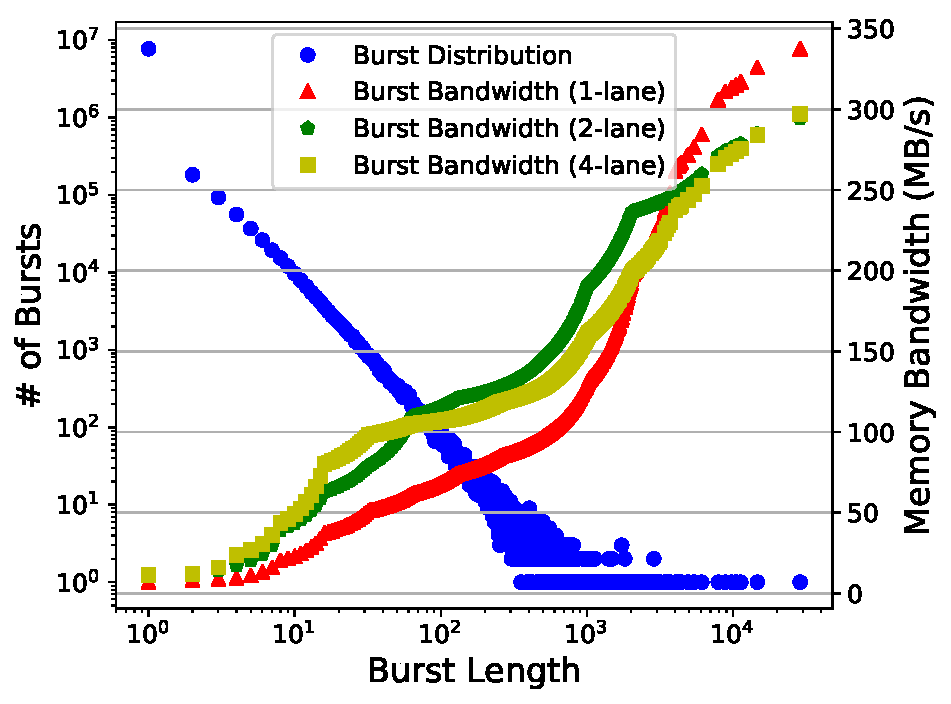
\includegraphics[width=0.75\linewidth]{burst_len_youtube}}
	\caption{Burst length distribution in BFS on Youtube Social Network Graph. 
		Random memory access and short sequential memory access take up the 
		the majority of the memory access overhead of BFS. Multiple parallel 
		lanes of data paths improve the memory bandwidth utilization when the 
		burst lenght is relatively large, but they will not help much 
	for short or random memory accesses.}
	\label{fig:burst-len-youtube}
	\vspace{-1.5em}
\end{figure}

\textit{Observation 2: There are many redundant vertices in the 
frontier vertex neighbors leading to a lot of redundant memory access in BFS.} 
As random memory access takes up a big portion of the overall memory 
access overhead, we further investigate the random memory access in BFS. 
According to the level synchronous BFS algorithm, the random memory access mainly comes 
from the frontier neighbor vertex status read/write. 
However, many frontier vertices may have common neighbor vertices and these common 
vertices lead to many repeated vertex statuses read. To gain insight of the neighbor 
vertex redundancy, we compare the total amount of frontier 
neighbor vertices and the amount of unique frontier neighbor vertices in each BFS iteration.
(Note that Youtube graph is used in the experiment.) 
The comparison is presented in Figure \ref{fig:repeat-neighbor} and it shows 
that there are considerable redundant vertices in BFS iterations. 
The redundancy proportion even goes up to 80\% in the BFS iteration with the most frontiers. 
With proper redundancy removal strategy, the vertex status reads in the following 
part of the BFS can be reduced dramatically.

On top of the redundant vertices, the visited vertices in previous 
BFS iterations do not need to be checked by reading the vertex status 
from memory. According to our experiment, the visited frontiers 
take up quite some of the total frontier neighbor vertices. However, this is 
observed in only one or two BFS iterations. Buffering 
frontier vertices may help to avoid unnecessary random vertex status read, 
but the benefit may be relatively trivial.  

\begin{figure}
	\center{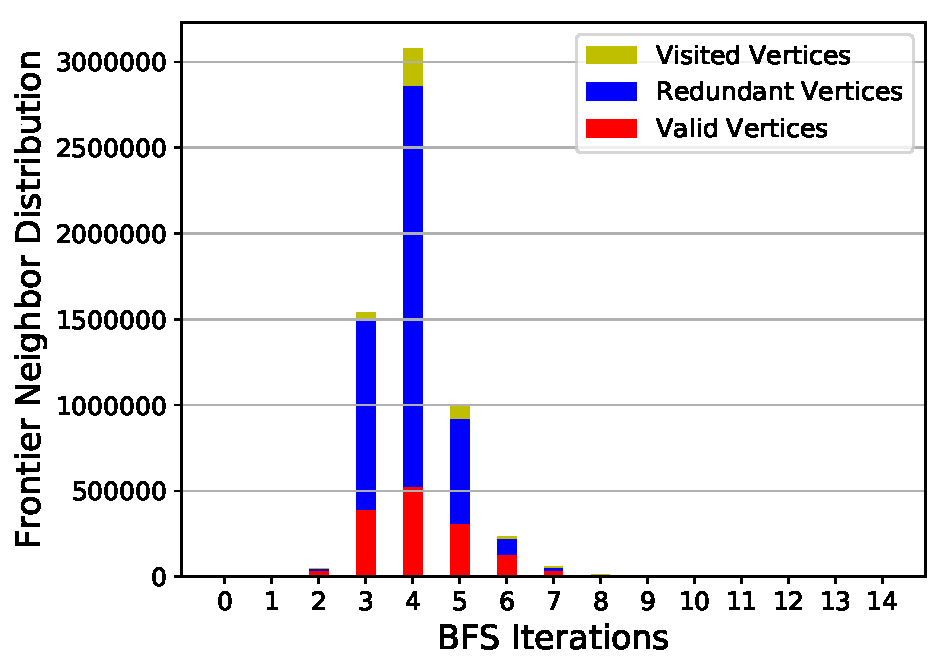
\includegraphics[width=0.75\linewidth]{neighbor_vertex}}
	\caption{Unnecessary random vertex status read decomposition. 
		The frontier neighbors consists of three parts including visited vertices 
		in previous BFS iterations (visited vertices), 
		redundant vertices that are repeatedly traversed in one BFS iteration (redundant vertices), 
		and the actual valid vertices that must be traversed (valid vertices). 
		The first two parts of the vertices can be ignored without 
	affecting the correctness of the BFS.}
	\label{fig:repeat-neighbor}
	\vspace{-1.2em}
\end{figure}

\textit{Observation 3: The vertex status reads have good 
	spatial locality especially when the redundant access is removed in advance, 
	but the temporal locality is relative bad meaning that the status reuse 
distance is quite long.}
Another potential optimization of random memory access is to use cache architecture, 
which explores the data locality and improves memory bandwidth utilization 
accordingly. To ascertain the feasibility of using cache, we analyze both the 
temporal and spatial locality of the vertex status reads. Since 
the frontier neighbor vertex redundancy removal affects the locality, 
we also do the spatial locality analysis on a redundancy-free 
vertex status read sequence. The data locality based cumulative 
distribution function (CDF) curve is shown in 
Figure \ref{fig:youtube-locality}. Clearly, the memory accesses exhibit 
very good spatial locality. In particular, the spatial 
locality gets even better and over 70\% of the vertices have reference distance 
less than 200 when the redundancy is squeezed. The temporal locality is not as 
good and only around 20\% of the accesses have short reuse distance. In general, 
we still believe that a specialized cache is beneficial to the random 
vertex status reads. Note that we use 
the stride distance as the metric of spatial locality and reuse distance as the metric 
of temporal locality \cite{weinberg2008chameleon}. The stride distance of a reference 
to address A is defined as the minimum distance between A and the 
memory addresses in a lookback window right before the current 
memory access. We set the loopback window to be 32 in the experiment. 
The reuse distance of some reference to 
address A is equal to the number of unique memory addresses that have been 
accessed since the last access to A.  

\begin{figure}
	\center{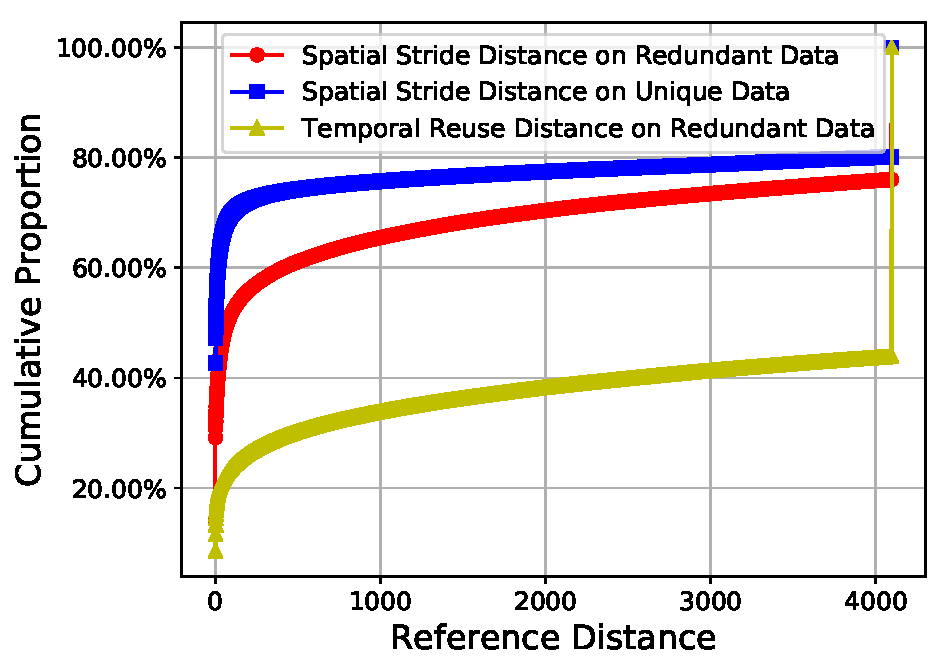
\includegraphics[width=0.75\linewidth]{youtube-locality}}
	\caption{Cumulative Distribution Function (CDF) of reuse distance 
		and stride distance. They stand for the temporal locality and spatial 
		locality of the BFS vertex status reads respectively. Note that the 
		accesses with reference distance larger than 4000 are combined as they are difficult 
	to be optimized in hardware design.}
	\label{fig:youtube-locality}
	\vspace{-1.5em}
\end{figure}

%\textit{Observation 4: In the skewed graphs, a small amount of high degree vertices 
%covers a big proportion of the connections (edges) in the graph.}
%The real-world graphs usually have large amount of vertices and adges while 
%the FPGA on chip memory is far from enough for caching and buffering. 
%Hereby, only a sub set of them can reside in on-chip memory at runtime. 
%It can be expected that high degree vertex related information 
%are more likely to be referenced in 
%the BFS iterations. To further investigate the potential of buffering 
%the high degree vertices, we analyzed the vertex degree distribution 
%of Youtube graph. The vertex degree based CDF and vertex based 
%CDF is shown in Figure \ref{fig:degree-distribution}. The two CDF curves in the figure 
%exhibit that the top 10\% high degree vertices include more than 70\% of 
%vertex degree namely edges in the graph. Basically keeping these high degree 
%vertex infomration such as vertex status on chip can avoid the repeated 
%vertex staus checking in BFS and is benefitial to the memory access efficiency. 
%Another thing that is worth for highlighting is the one degree vertex distribution.
%It takes up over 40\% of the overall amount of the vertices in the graph. In BFS, 
%the status of these vertices will be read and write only once.  
%
%\begin{figure}
%\center{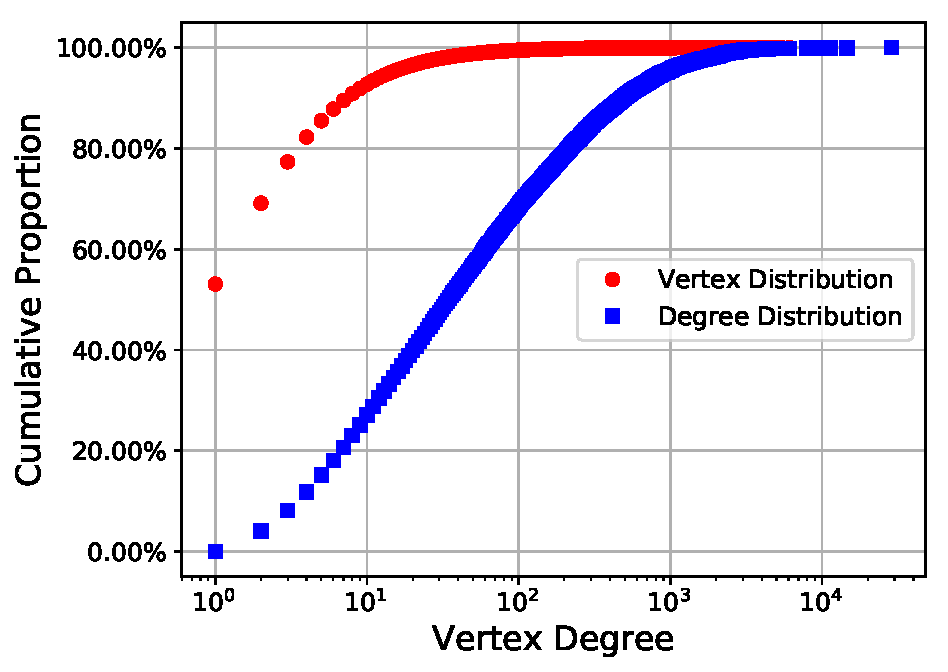
\includegraphics[width=0.9\linewidth]{degree-dist}}
%\caption{Vertex Degree Distribution. A small amount of 
%    high degree vertices take up a large portion of the connections in the graph.}
%\label{fig:degree-distribution}
%\end{figure}

In summary, we notice that random and short sequential memory accesses 
are the most time-consuming part of the overall BFS memory accesses. 
It is generally difficult to optimize these memory accesses, 
With intensive experiments, we observe a large amount of redundancy in BFS and 
these memory accesses exhibit very good spatial locality. Taking advantage of the 
memory access characteristics, we may improve the BFS memory access efficiency 
and performance eventually.

\section{BFS Accelerator Overview} \label{sec:overview}
\textcolor{green}{This work targets at in-memory graph processing on a PCIe based 
high-performance FPGA card. The whole graph is stored in FPGA device
memory. Ideally, the accelerator does the BFS on FPGA without
any interference from the host CPU. However, the data flow model 
of Xilinx HLS does not allow feedback from the downstream stages 
to previous stages. In this case, we actually implement one 
BFS iteration on FPGA while leaving the host CPU to do the iteration 
control. The BFS kernel on FPGA returns the BFS frontier size to host such 
that the host can decide if BFS completes. Although communication 
between the host and FPGA in each BFS iteration is required, the communication cost 
is negligible compared to the execution time and the overall BFS runtime 
is barely affected.}

The BFS algorithm is critical to the BFS accelerator 
and level synchronous BFS is widely used.  
However, it may have redundant vertices pushed to the 
frontier queue in a parallel architecture. The redundancy 
vertices are difficult to get rid of \textit{completely},
\textcolor{red}{while they may lead to a large 
number of repeated traverses recursively and degrade the BFS performance.
To address this problem, we inspect the frontier from the 
vertex status in each BFS iteration to cut down the 
propagation of the redundancy. The modified algorithm is described 
in Algorithm \ref{alg:modified-bfs}. Instead of traversing the frontier vertices directly, 
it starts with vertex status traverse and inspects the frontier 
in each BFS iteration. The inspection processing are complete sequential 
memory access and can be done efficiently and it helps to remove 
the redundant frontier vertices completely.} The rest part of the algorithm is 
quite similar to the level synchronous BFS except that the frontier queues 
are no longer needed.

\begin{algorithm}
	\caption{Modified BFS Algorithm} \label{alg:modified-bfs}
	\footnotesize
	\begin{algorithmic}[1]
		\Procedure{BFS}{}
		\State $level[v_k] \gets -1$ where $v_k \in V$
		\State $level[v_s] \gets 0$, $current\_level \gets 0$, $frontier \gets v_s$

		\While {$!frontier.empty()$} 

		\For{$v \in V$}
		\If{$level[v] == current\_level$}
		\State $frontier \gets v$
		\EndIf
		\EndFor

		\For{$v \in frontier$}
		\State $S \gets {n \in V | (v, n) \in E}$
		\For {$n \in S$}
		\If {$level[n] == -1$}
		\State $level[n] \gets current\_level + 1$
		\EndIf
		\EndFor
		\EndFor
		\State $current\_level \gets current\_level + 1$
		\EndWhile
		\EndProcedure
	\end{algorithmic}
\end{algorithm}

\section{HLS based BFS optimization} \label{sec:bfs-opt}
With the observations in Section \ref{sec:observation} 
and the modified BFS algorithm in Section \ref{sec:overview}, 
we start to optimize the BFS accelerator using high-level design tools 
from different angles. First, we convert the nested loop structure 
of the BFS to be a streaming manner such that it can be fit into the data flow model in
Xilinx HLS for efficient pipelined execution. Then we explore a series of memory optimization 
techniques based on the BFS memory access patterns observed in \ref{sec:observation}. 
Afterwards, we apply some general HLS optimizations to the resulting design. Finally, 
we tune the design parameters such as the prefetch buffer size and cache size through 
the software emulation and provide optimized configurations for each graph data set.

\subsection{BFS pipelining}
We divide the BFS algorithm into pipelined 
sub functions as summarized in Figure \ref{fig:bfs-stream}. 
The six sub functions are labeled as \textit{f1} to \textit{f6} respectively. In \textit{f1}, 
vertex status is read from FPGA DDR memory sequentially through a streaming port. 
When the vertex status is fetched, \textit{f2} inspects the status 
flowed from the stream buffer, decides the current frontier 
and dumps the frontier to the downstream pipeline. 
With the frontier stream, \textit{f3} can further fetch graph 
data stored as CSR. CSR includes a row pointer array (RPA) 
and a column index array (CIA), and they must be sequentially accessed. 
In \textit{f3}, we combine each pair of RPA entry of the frontier as a construct 
and pass it to the next stream function \textit{f4}. When \textit{f4} gets the RPA pair, 
it can read the CIA sequentially through a streaming port. 
When data in CIA stream which is essentially the potential 
next frontier vertices are received in \textit{f5}, their vertex status 
will be checked by reading the vertex status array stored in DDR as well.
Only the vertices that are not visited yet will be further forwarded to the \textit{f6}. 
In \textit{f6}, the vertex status will be updated.

In the streamed BFS implementation, five sub-functions involve external memory access 
and they have quite different memory access patterns. \textit{f3} reads all the vertex 
status and it is essentially a long sequential memory read. \textit{f2} reads the CSR 
row pointer of the frontier. Two sequential words will be read each time. 
\textit{f1} reads the CSR column index and the 
burst length depends on the vertex degree which varies in a large range. 
\textit{f4} and \textit{f5} involve vertex status reads and writes of the next frontier vertices.
As these vertices are not sequential, the HLS tools just take them as random access. 

\begin{figure}
	\center{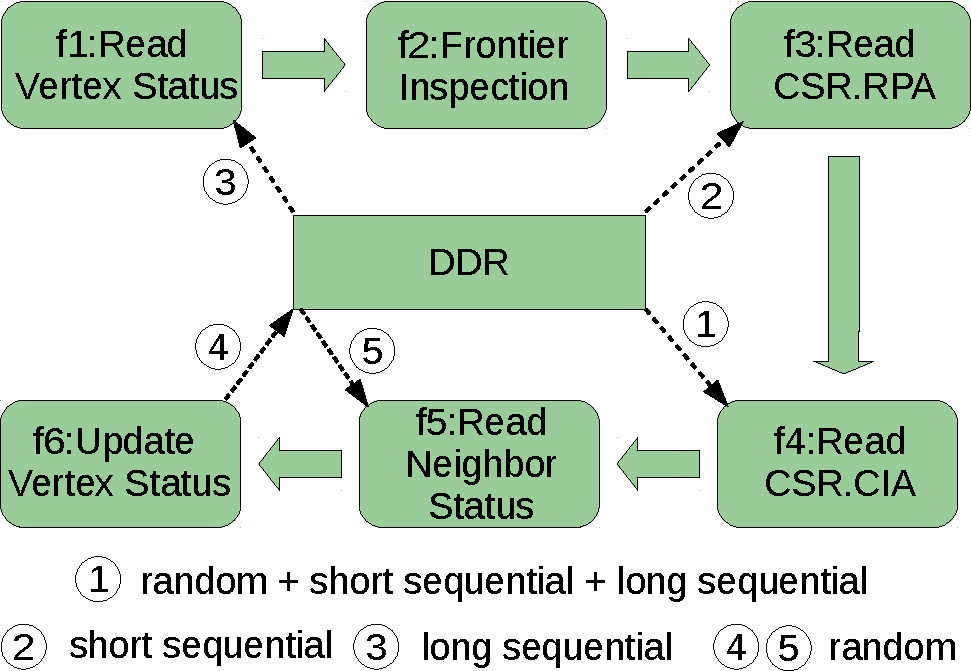
\includegraphics[width=0.65\linewidth]{bfs-stream}}
	\caption{Streamed BFS Algorithm}
	\label{fig:bfs-stream}
	\vspace{-1.5em}
\end{figure}

\subsection{Memory Access Optimization}
In this section, we mainly explore the memory 
access optimization techniques based on the observations 
in Section \ref{sec:observation}.

\subsubsection{Redundancy Removal}
There are many redundant vertices among the frontier neighbors in BFS. 
In order to remove the redundant memory access, we create hash tables 
to perform the redundancy removal. As the redundant vertices are 
relatively random, a big hash table can be utilized to squeeze 
the redundancy. However, big hash table degrades the hardware implementation 
frequency and eventually lowers the overall performance. Hereby, we 
build a series of smaller hash tables and apply them in parallel. 

\subsubsection{Caching}
According to the experiments in Section \ref{sec:observation}, 
there are many random memory accesses and short 
sequential memory accesses in \textit{f5} and \textit{f6}. 
It is generally difficult to optimize these memory accesses. Fortunately, 
the spatial locality analysis shown in previous section 
implies the great potential of cache-based memory access optimization. 
Inspired by the observation, we developed an HLS based cache specifically 
for the vertex status \textit{depth} access. 

Since the cache is only used for \textit{depth} array read and write, we  
choose the \textit{depth} array index instead of its physical address for cache 
indexing. As the cache cannot be shared 
between different SDAccel data flow functions, a natural cache design is 
to implement both cache in \textit{f5} and \textit{f6}. The cache can be relatively simple 
for supporting only read operations in \textit{f5} and write operations in \textit{f6}.  
In this work, we choose the directly mapped cache considering the hardware implementation.  

\subsubsection{Prefetching}
According to the BFS algorithm, the frontier is sequentially inspected. 
Therefore, the CSR information is also accessed in a single direction 
in \textit{f3} and \textit{f4}, though they are not necessarily sequential. Basically 
both the column array index and the row array index will increase 
monotonically in each BFS iteration. The CSR data will not be repeatedly 
referenced through the BFS. To optimize these memory 
accesses, a small prefetch buffer is built to improve the memory access efficiency. 
We notice that 64-byte prefetch buffer provides reasonable hit rate and 
it is used in the experiments.

\subsection{General HLS optimization}
On top of the BFS specific optimizations, there are also 
some other relatively general design optimizations that can improve the 
resulting BFS accelerator performance. These optimizations will be briefly 
introduced in this subsection.

\subsubsection{Memory bank-aware data layout}
The data layout affects the memory access efficiency 
especially for multiple-bank DDR memory, we thus explore the 
data layout of the graph for higher memory bandwidth utilization. 
Graph is typically stored as CSR which has two arrays i.e. the row pointer 
array (RPA) and column index array (CIA). A straightforward way that 
divides the two arrays into multiple memory banks is inefficient (i.e. using higher bits of the 
address as the bank selection signal), because a vertex's neighbors may stay in different 
banks and traversing this vertex requires accessing all the different memory banks. 
As a result, each processing stage must include all the memory ports attached 
to the different memory banks and the hardware implementation will be expensive 
in SDAccel. To solve this problem, we reorganize the CSR data such that the 
time-consuming BFS pipeline stages including \textit{f3}, \textit{f4}, \textit{f5} and \textit{f6} 
can be split and parallelized. Each split of the processing can operate 
on just one memory bank, which makes the hardware design more efficient.

The detailed data layout including both the \textit{depth} and 
CSR is shown in Figure \ref{fig:csr-layout}.
The \textit{depth} is spread evenly across the memory banks 
with the granularity of 64 elements. The fine-grained partition 
granularity ensures the load balance of the processing on 
different memory banks. The \textit{RPA} of the CSR is partitioned 
with the same manner. To ensure aligned RPA access, we change the 
RPA structure with two arrays. One of the arrays stores the start \textit{CIA} 
index of each vertex and the other array stores the vertex's neighbor size.
The \textit{CIA} array is allocated to different memory banks 
based on the \textit{RPA} partition. Basically, we want to ensure that each vertex's 
neighbors stay in the same bank with its \textit{RPA}. However, when a frontier's neighbors 
are read into FPGAs, the \textit{depth} update process i.e. \textit{f6} may still need to refer to multiple 
\textit{depth} banks. We solve this problem by adding an additional crossbar stage on FPGA and 
reshaping the \textit{depth} updating streams to independent memory banks. Similar methods 
can be applied in \textit{f3}, so the partitions of different arrays can be different.
In this work, \textit{depth} is divided into two memory banks 
while CSR data are divided into 4 memory banks considering the 
amount of memory accesses and the total amount of memory port constrain in SDAccel.

\begin{figure}
	\center{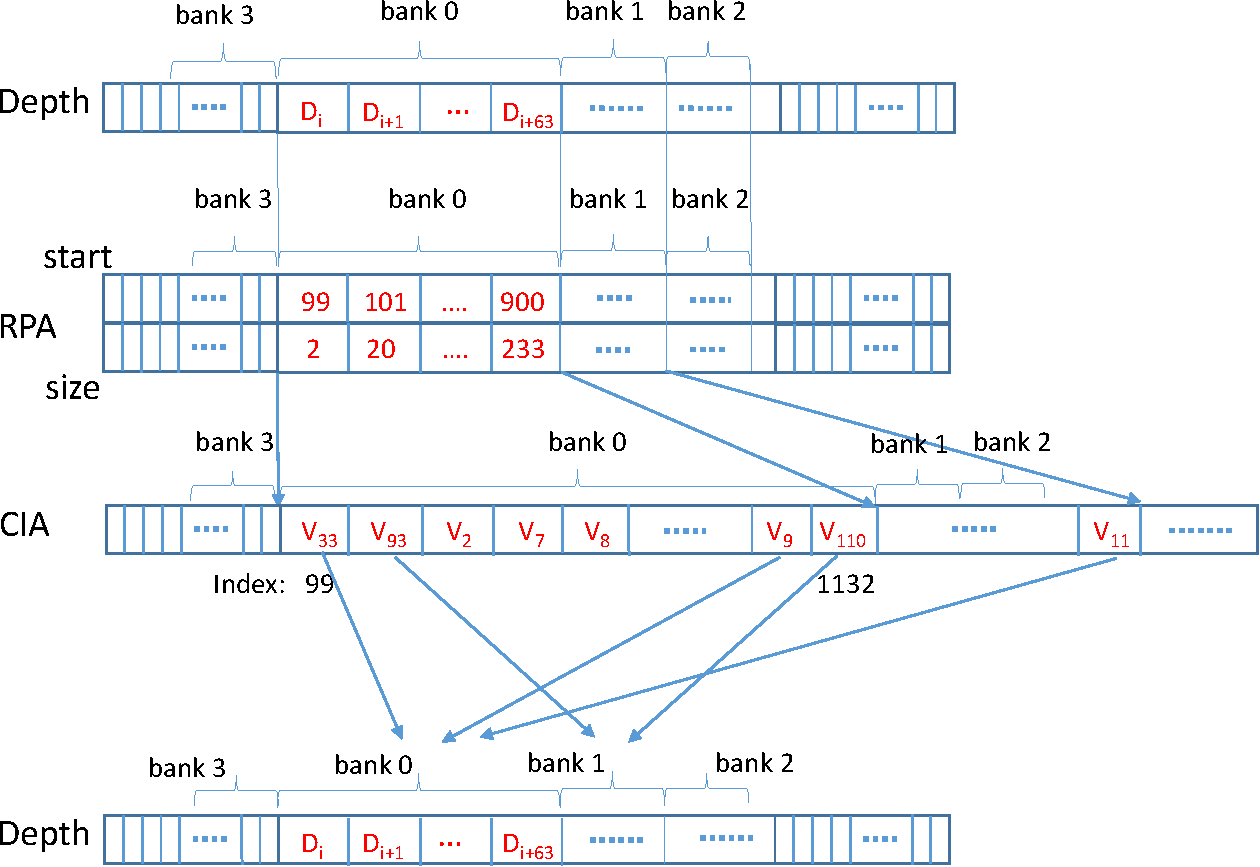
\includegraphics[width=0.85\linewidth]{csr-layout}}
	\caption{BFS data layout on multiple-bank DDR memory.}
	\label{fig:csr-layout}
	\vspace{-1em}
\end{figure}


\subsubsection{Data path duplication}
When the DDR memory bandwidth is not saturated, a simple 
yet efficient optimization method is to duplicate the data paths. 
With multiple parallel BFS data paths, the accelerator can issue more parallel 
memory requests pushing higher memory bandwidth utilization. A straightforward 
way of data path duplication is to split the vertex status into different 
partitions and each partition is processed by an instance of the same BFS data path.
However, this method may not work as good as expected, because 
the vertices in the frontier may not distribute evenly across the graph. 
and the different data paths may have unbalanced workloads. Also it requires 
more global memory ports when the data paths are duplicated.

To address the problems, we propose a delicate data path duplication strategy 
as shown in Figure \ref{fig:duplicate-pipeline}. According to the BFS algorithm, 
we know that each frontier vertex requires two CSR row pointer read and multiple 
CSR column index read. Thus the bottleneck pipeline stages may probably start 
from \textit{f3}. Therefore, we split the frontier stream generated in \textit{f3} into 
multiple streams. Each sub-stream will be handled independently by a 
duplicated data path. This also solves the data path load balancing problem 
naturally. Finally, to ensure both parallel memory access and cache coherence,  
we reshape the output streams of \textit{f5} into multiple independent streams 
with a crossbar logic such that data in each stream will not overlap 
and there is no memory write conflicts. 

\begin{figure}
	\center{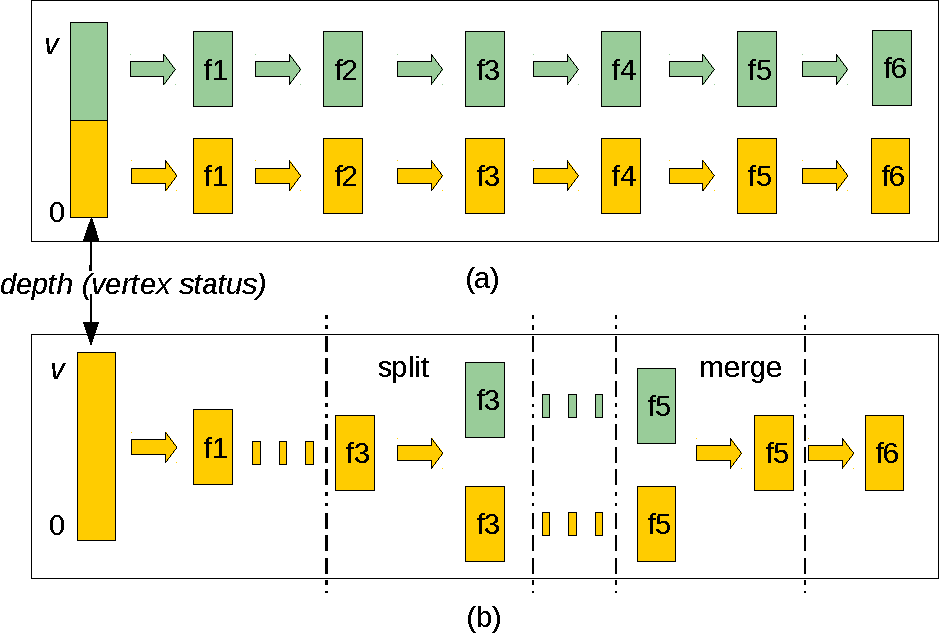
\includegraphics[width=0.75\linewidth]{pipeline-duplication}}
	\caption{pipeline duplication. (a) straightforward pipeline duplication 
	(b) optimized pipeline duplication.}
	\label{fig:duplicate-pipeline}
	\vspace{-1.5em}
\end{figure}

With this data path duplication strategy, each pipeline stage of a data path typically 
operates on an independent set of the data. When the design is implemented on 
an FPGA with multiple memory banks, each data partition can be mapped to a single memory bank.
The data path duplication scheme makes it convenient to explore the multiple-bank 
memory bandwidth. It is fine to create more parallel data paths than the amount of the memory 
banks, but the total amount of global memory ports is limited to 16 in SDAccel. As a result, 
limited pipeline stages can be duplicated. 

\subsubsection{Data width optimization}
The memory bandwidth utilization is sensitive to the data width setup. 
Sequential memory access with 512-bit data width achieves the optimal 
memory bandwidth utilization \cite{kalms2017exploration}.  
With this guideline, the design parameters such as the cache line size 
and prefetch length are set to be 512-bit. For sequential 
memory access, they are aligned and accessed with 512-bit memory port.

%\subsubsection{II optimization}
%In the pipelined design, initialization interval (II) indicates the 
%processing throughput. Larger II in a single pipeline stage 
%may slow down the rest of the system. Thus we try to reduce II of all 
%the pipelined sub-functions. In particular, hash table, cache and prefetch 
%buffer may affect the II. Inappropriate implementation may lead to 
%large II and even compensate the benefits brought by these optimizations. 

\subsubsection{Deadlock removal}
Another challenge of the pipelined BFS accelerator design is the 
unexpected deadlock problem. 
When a pipeline stage issues a burst request to the memory 
but gets stalled due to the insufficient read buffer, it has to 
wait for the downstream pipeline stages to consume the data in the buffer. 
However, the downstream pipeline stages may also be stalled due to 
the failure of acquiring the bus that is taken by the upstream pipeline stage.
It is difficult to debug and resolve this deadlock. To address this problem, we
add an additional local buffer in the pipeline stages with long sequential 
memory access and split the long sequential memory access into smaller 
segments such that each segment can be accommodated by the buffer. 
Although this may cause slightly lower bandwidth utilization, it breaks the deadlock and 
ensures the correctness of the pipelined design.

\subsection{Parameter Tuning}
As presented in previous sub-sections, there are some design 
parameters such as hash table size and cache configurations
that need to be explored. \textcolor{red}{However, exploring all the design parameters 
based on the hardware implementation directly is extremely time-consuming, 
because a typical hardware implementation may take hours to complete the compilation.}

In this work, we tune the design parameters through the software 
emulation based analysis. We extract a series of 
implementation independent metrics such as cache hit rate and hash table hit rate 
through convenient software emulation of the HLS design. 
\textcolor{red}{With these metrics, we can decide the design parameters such as prefetch buffer size, 
cache size, and hash table size etc. Since software emulation allows very fast 
parameter exploration, we consider all possible combinations of 
those parameters and choose the optimal configuration that leads to the best performance. }

%\subsection{Parameter tuning}
%In this work, we manually tune the design parameters. To obtain the 
%optimized design parameters rapidly, we proposed a general HLS design 
%parameter tuning flow for the HLS based design. The design flow is 
%presented in Figure \ref{fig:parameter-tuning}. It includes three 
%iterative loops tuning different types of the design parameters.
%
%The first loop replies on the fast software emulation which is 
%immediately available using HLS.
%With the software emulation, we can extract a set of statistical 
%metrics such as cache hit rate, prefetch hit rate that are 
%mostly independent with the hardware implementation. These metrics can be used to 
%guide the cache and prefetch buffer design. Although they 
%are not sufficient to decide the exact accelerator performance, they 
%can help prune the design options that are far from optimal and thus reduce 
%the design parameter tuning time. The second tuning loop is based on the hardware 
%pre-synthesis which is also fast and can be done in a few minutes. 
%With the pre-synthesis report, we can optimize the II by 
%improving the HLS design. When the potential design 
%configurations gets smaller, we can get into the last loop and start the time consuming 
%hardware implementation evaluating the configurations with the real 
%performance or resource metrics. Finally, we would like to emphasize the verification process, 
%it needs to be enabled all the time, as optimization may also cause mistakes of the resulting design.
%
%\begin{figure}
%\center{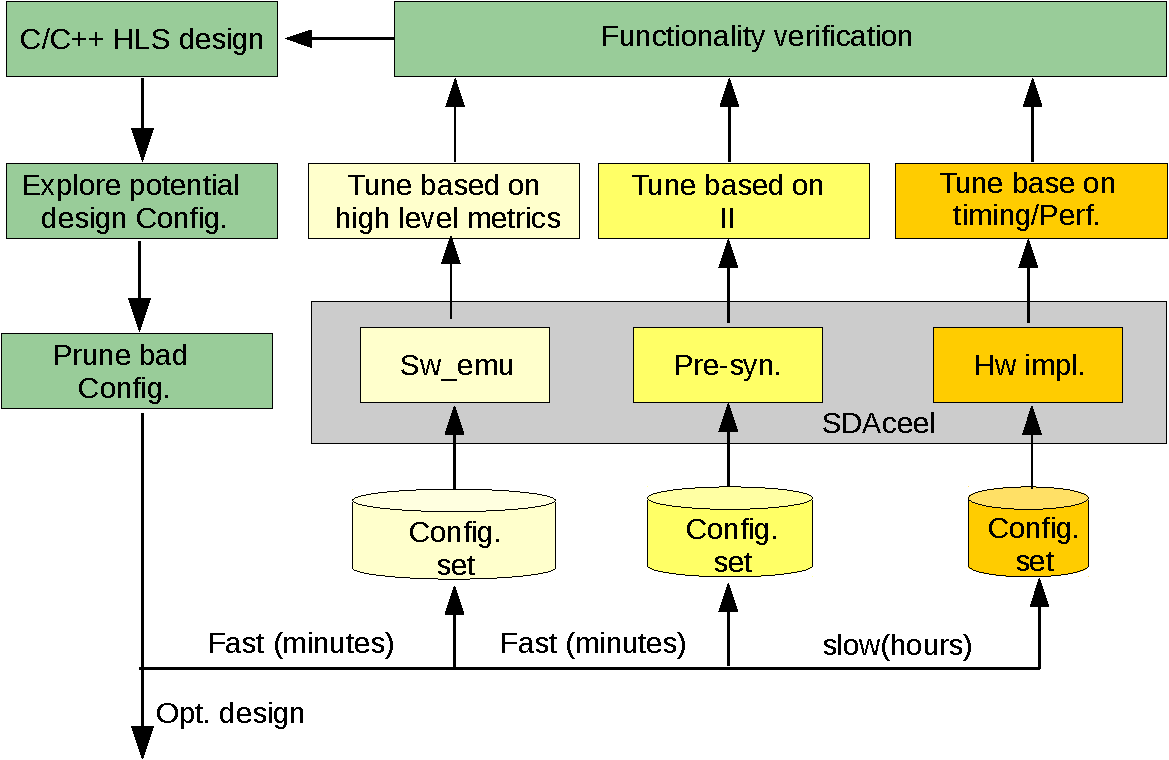
\includegraphics[width=0.95\linewidth]{parameter-tuning}}
%    \caption{Design parameter tuning flow based on SDAccel.}
%\label{fig:parameter-tuning}
%\end{figure}
%

%\appendix
%\section{Acknowledgement}

%\begin{acks}
%  The authors would like to thank Sam Ho for providing the suggestions on
%  HLS design debugging and optimization as well as the SDAccel usage. 

%\end{acks}



\bibliographystyle{ACM-Reference-Format}
\bibliography{refs} 

\end{document}
